\section{A Javadoc Extension for API Contracts}
\label{sec:approach}

%update to be more general
\contractjdoc{} for Java is an extension to the Javadoc-tagging systems with
contracts surrounded by brackets. Its compiler
extends AspectJML~\cite{aspectjml}, with support for runtime checking.
\contractjdoc{} allows programmers to document precise source code's behavior as
part of Javadoc commentary. With just a few new tags, in addition to the
standard Javadoc tags, one can write contracts as Javadoc comments that are
compiled to runtime checkable code.
The \contractjdoc{} approach fulfills the gap between informal documentation
(as with Javadoc) and formal specification (such as JML~\cite{jml} or
Code Contracts~\cite{codeContractsPaper}).

In the remaining of this section, we present how \contractjdoc{} supports Java code
documentation with both informal and formal features of the documentation
approaches discussed in Section~\ref{sec:example}. The presentation is
informal and based on our running example.

\subsection{\contractjdoc{} Design for Java}

We define \contractjdoc{} constructs as traditional Javadoc tags which are embedded within
block comments. The main idea is to allow a mix between the traditional Javadoc
syntax and JML. This mix is used to tackle the dilemma explained in the end of
Section~\ref{sec:example}.

Embedding contracts means expressing specifications
(e.g., preconditions) in the existing Javadoc comments
and making them machine discoverable through the use of
marker brackets within those comments.
Advantages of embedding a contract language are that
programmers do not need to learn a new specification language.
This is specially true because the overwhelming majority of contracts that programmers write in
practice are short and simple~\cite{Estler-etal14,typeContracts}.
For instance, 75\% of Code Contracts~\cite{codeContractsPaper} projects,
the written contracts are basic checks for the presence of data
(e.g., non-null checks)~\cite{typeContracts}. For scenarios like these,
there is no additional effort in embedding such contracts in Javadoc comments
using our \contractjdoc{} approach.

\subsubsection{Documenting Preconditions}
Recall the precondition illustrated in Section~\ref{sec:example}.
We discussed two ways to document such a precondition, a formal
one in JML (see Figure~\ref{Fig-JML-Bank}) and an informal one with
plain Javadoc comments (see Figure~\ref{Fig-Javadoc-Bank}).
In \contractjdoc, that precondition can be rewritten to the
following:
\begin{lstlisting}[basicstyle=\footnotesize\ttfamily,name=figxpi, frame=lines, mathescape=true]
 /**
  * @param amt the amount value to withdraw, 
  *   where $\shd{[amt > 0 \&\& amt <= balance]}$
  */
 double withdraw(double amt) 
   throws TransactionException {...}
\end{lstlisting}
Tag \lstinline!@param! documents parameter \lstinline!amt! of \lstinline!double! type.
Besides the usual comments, we have added a Java-like boolean expression
surrounded by brackets; these brackets indicate assertions internally in our
tool; \contractjdoc{} compiles the above Javadoc comments into an executable
precondition checking.
An alternative (not showed) is to replace tag \lstinline!@param!
by \lstinline!@requires! or \lstinline!@pre!. Both can be used
to document a precondition constraint; the main difference is that
they are not part of the standard Javadoc tagging system.

\subsubsection{Documenting Postconditions}
A postcondition expresses the obligations of a supplier (and
respectively the rights of a client), specifying the result of a method.
As discussed in Section~\ref{sec:example}, two kinds of
postconditions are usually found in Javadoc and JML, one related to normal return, and another related to
exceptional return. Let us use \contractjdoc{} to document postconditions:
\begin{lstlisting}[basicstyle=\footnotesize\ttfamily,name=figxpi, frame=lines, mathescape=true]
 /**
  * @return amt the current balance after withdraw,
  *   that is $\shd{[@return == balance]}$
  * @throws TransactionException the 'balance' does
  *  not change, that is $\shd{[balance == @old(balance)]}$
  */
 double withdraw(double amt) 
   throws TransactionException {...}
\end{lstlisting}
Tags \lstinline!@return! and \lstinline!@throws! document
the two kinds of postcondition, with their respective assertions
expressed within brackets. Note that both use two special tags within
the assertion brackets. Tag \lstinline!@return! appears again within
the brackets. This inner is allowed (in \contractjdoc{}) and allows one
to use the value of the method's  returns to write the contract regarding
the normal postcondition. A similar tag, \lstinline!@result! derived from the JML syntax,
can also be employed instead of the inner use of the \lstinline!@return! tag.
Moreover, tag \lstinline!@old! (also derived from JML) refers to
expressions or fields in their pre-state. This tag can only be used
by the Javadoc tags related to postconditions.

As with preconditions, \contractjdoc{} offers three tags for expressing postconditions.
For normal postconditions, the similar JML-based tags \lstinline!@ensures!
and \lstinline!@post! can be used in place of the standard one \lstinline!@return!.
In relation to the \lstinline!@throws! tag, the standard Javadoc offers a surrogate tag
\lstinline!@exception!. Derived from JML, we can also employ
the \lstinline!@signals! tag to document and constrain exceptional behavior.


\subsubsection{Documenting Invariants}

Beyond the support for pre- and postconditions, \contractjdoc{} make the use of invariants also
available by means of \texttt{@inv} tags.
The format of writing is the same as those
for pre- and postconditions.
The difference is related to the semantics: while pre- and postconditions apply to a specific
method, an invariant applies for all methods from a class. For invariants, we follow the
semantics of the JML language. For more information, please refer
to~\cite{jml}.
The invariant contract, described in Section~\ref{sec:example}, can be written
as follows:
\begin{lstlisting}[basicstyle=\footnotesize\ttfamily,name=figxpi, frame=lines, mathescape=true]
class BankAccount {
 /**
  * @inv The overall balance should be $\shd{[balance >= 0]}$
  */
 double balance;
 //...
}
\end{lstlisting}
Invariant declarations may be placed above the field
declarations (as in the example), or  above the
class declaration as a valid Javadoc block comment.

\subsection{\contractjdoc{}'s Supporting Infrastructure}

We implemented the \contractjdoc{} compiler in the top of
the open source AspectJML/ajmlc compiler~\cite{aspectjml,ajmlc,Rebelo-etal08}.
Unlike the original JML compiler (jmlc), ajmlc presents code
optimizations and improved error reporting~\cite{ajmlc}.
Differently from jmlc, AspectJML also enables the modularization
of crosscutting contracts that can arise in standard
JML specifications~\cite{aspectjml}.

We adapted the front-end of the AspectJML/ajmlc compiler
to convert/preprocess
the \contractjdoc{} tags into the corresponding JML
features, like pre- and postconditions.
After conversion, the compilation occurs as usual and
generates aspects to runtime checking the
contracts. See Figure~\ref{fig:compilerInfra}
for an overview of the compilation strategy.


\begin{figure}[h]
\centering
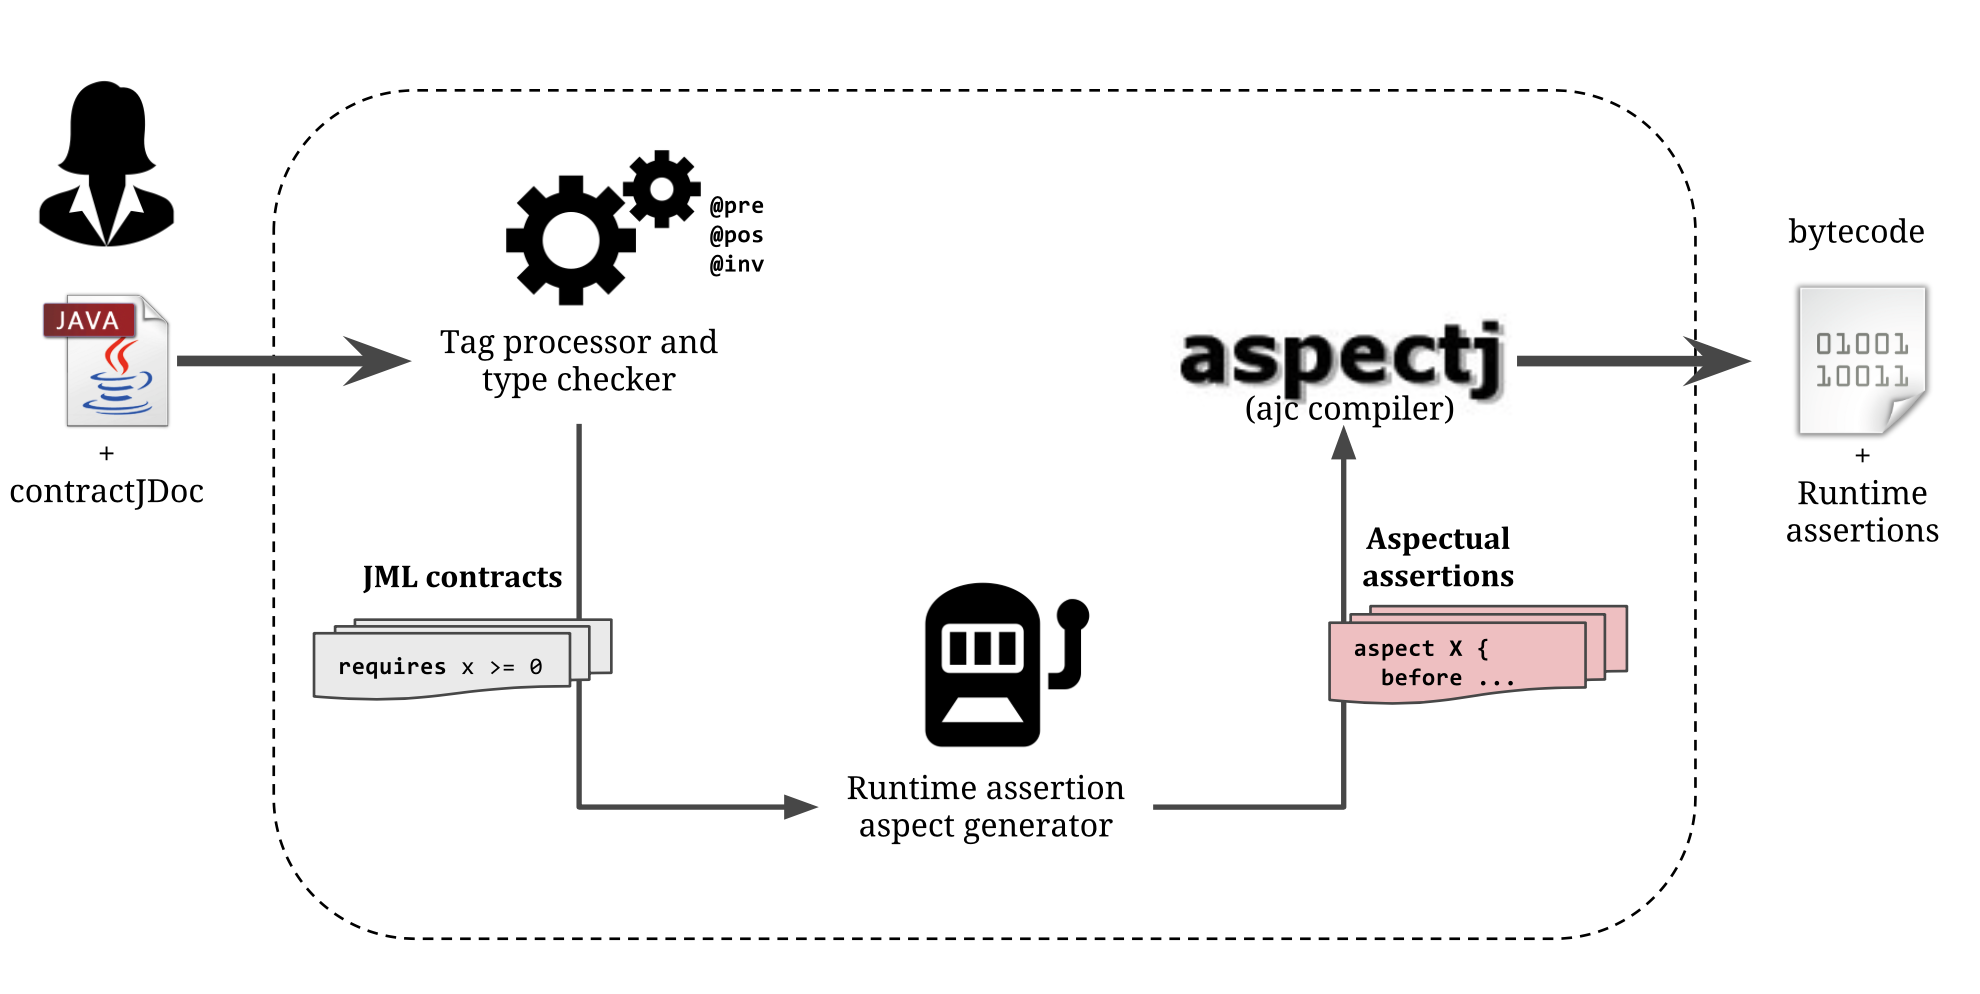
\includegraphics[width=1.0\textwidth]{figs/compilerInfra}
\caption{ContractJDoc Compilation. First, a source code with \contractjdoc{}
contracts passes through a tag processor and type checker. Then, the assertions
generated are runtime checked and AspectJ compiler produces a bytecode with
assertions.}
\label{fig:compilerInfra}
\end{figure}

